\chapter{Luca}

\begin{enumerate}
	\item \sd, go right and up to the next screen, \cs[2:30]. Don't save.
	\item \sd\ in locker room. Don't do the tutorial. \sd by mashing another button (like \textbf{R1}) at the same time as confirm, walk down, \sd
	\item Walk down to next screen, \sd. Whistle \cs[0:30], walk right to next screen.
	\item \sd, run to the cafe. \sd, \skippablefmv+\cs[1:20], \sd
	\item Run left to next screen, then left to the docks. Run north to the next screen.
\end{enumerate}
\begin{battle}{Machina}
	\begin{itemize}
		\item \textit{For the first two encounters:}
		      \begin{itemize}
			      \tidusf Defend
			      \kimahrif Defend
			      \luluf Thunder
		      \end{itemize}
		\item \textit{For the third encounter:}
		      \begin{itemize}
			      \item \textit{First Wave}
			            \begin{itemize}
				            \tidusf Attack
				            \kimahrif Attack
				            \luluf Thunder a different Machina
				            \tidusf Attack
				            \kimahrif \od\ Seed Cannon \textit{if no crits else} Attack
			            \end{itemize}
			      \item \textit{Second Wave}
			            \begin{itemize}
				            \tidusf Defend
				            \kimahrif Defend
				            \luluf Thunder
			            \end{itemize}
			      \item \textit{Third Wave}
			            \begin{itemize}
				            \tidusf Attack
				            \kimahrif Attack or \od\ Seed Canon
				            \luluf Thunder a different Machina
			            \end{itemize}
		      \end{itemize}
	\end{itemize}
\end{battle}
\begin{enumerate}[resume]
	\item If anyone is Critical HP, use Potions.
	\item Do the below Sphere Grid if \tidus\ has 5 S.Levels.
	\item Run right. 
\end{enumerate}
\begin{battle}[3000]{Oblitzerator}
	\begin{itemize}
		\kimahrif Defend
		\tidusf Defend \textit{If No Early Haste Else} Haste \lulu
		\luluf Thunder Crane x3
		\tidusf Use Crane after \lulu's string
		\kimahrif Defend
		\luluf Thunder
		\tidusf Attack
	\end{itemize}
	Check for \textbf{Lightning Steel, Thunder Ball}
\end{battle}
\begin{enumerate}[resume]
	\item \cs[2:00], \sd\ during and after Blitzball game.
\end{enumerate}
\vfill
\begin{spheregrid}
	\begin{itemize}
		\tidusf (5 S.Lvl)
		\begin{itemize}
			\item Move $\downarrow \searrow\searrow$
			\item +1 Str, Haste, +20 MP
		\end{itemize}
	\end{itemize}
	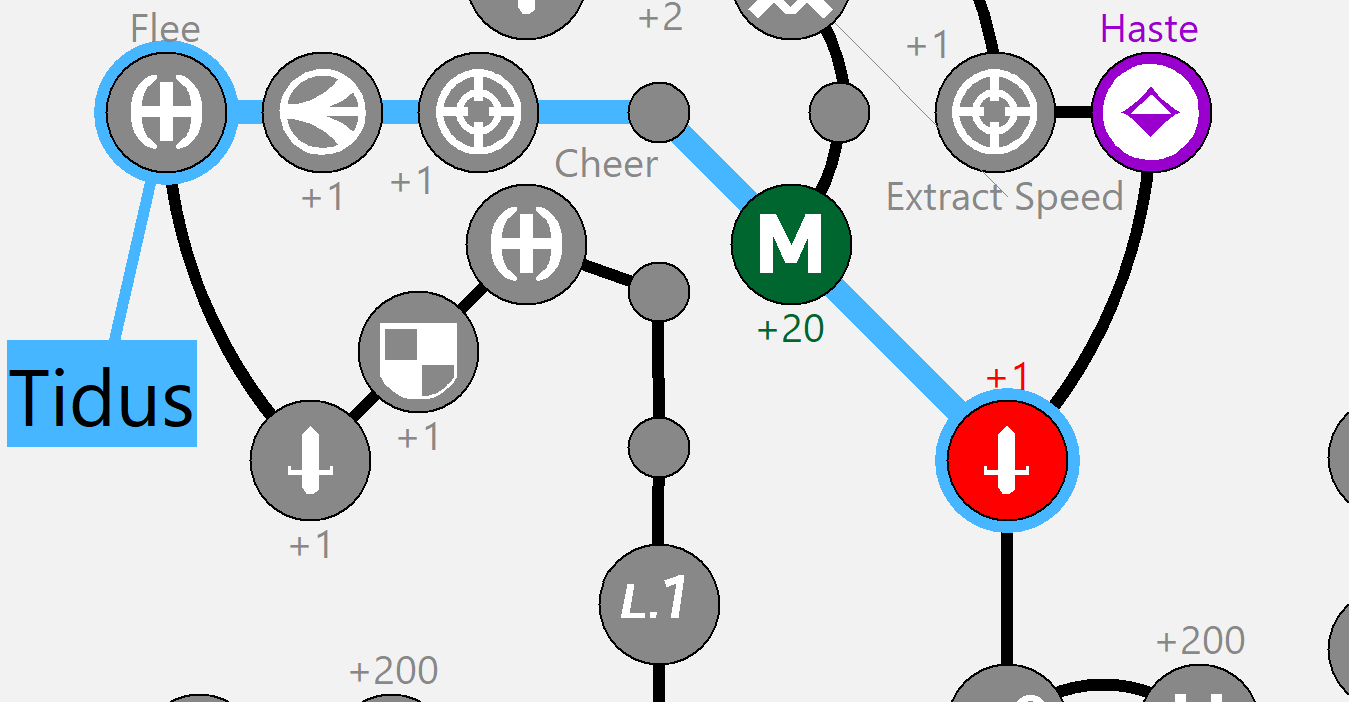
\includegraphics{graphics/haste}
\end{spheregrid}
\begin{enumerate}[resume]
	\item Auto-Sort items
\end{enumerate}
\begin{equip}
	\begin{itemize}
		\item \textit{If you got Lightning Steel}
		      \begin{itemize}
			      \tidusf Lightning Steel
		      \end{itemize}
		\item \textit{If you got Thunder Ball}
		      \begin{itemize}
			      \wakkaf Thunder Ball
		      \end{itemize}
	\end{itemize}
\end{equip}
\begin{enumerate}[resume]
	\item Run South for the next two screens. \save. Go up the stairs to the locker room, \sd
	\item Go back into locker room, speak to \wakka, \sd, \cs[1:20]. \sd\ after \lulu\ scene. \cs[1:40] on Auron Entrance.
\end{enumerate}
\vfill
\begin{blitzball}
	\begin{itemize}
		\item \textbf{First Half:}
		      \begin{itemize}
			      \item \textit{If Luca wins the Blitzoff:}
			            \begin{itemize}
				            \item Triangle, switch the mode to \textbf{Mark Mode}, and then \textbf{Left Side}
			            \end{itemize}
			      \item \textit{When you get the ball:}
			            \begin{itemize}
				            \item Change to \textbf{Manual A} and \textbf{Normal Mode}
				            \item down some, pass the ball to \tidus
				                  \tidusf Swim next to Jassu, pass to Jassu
				            \item Hide behind the Goalie
				            \item If you aggroed a Goer, Swim Around
			            \end{itemize}
		      \end{itemize}
		\item \sd\ during half time
		\item \textbf{Second Half:}
		      \begin{itemize}
			      \item \textit{If Luca wins the Blitzoff:}
			            \begin{itemize}
				            \item Triangle, switch the mode to \textbf{Mark Mode}, and then \textbf{Right Side}
			            \end{itemize}
			      \item \textit{When you get the ball:}
			      \item Pass to Jassu if he doesn't have it
			      \item Swim to the Bottom Middle
			      \item Wait until 2:20, if Abus Aggros then Break
			      \item Swim to the Left, aggro Balgerda (bottom player), then swim back some
			      \item Pass to \tidus\ before Balgerda gets in range to block
			            \tidusf Swim close to the Goal and Sphere Shot before anyone is close enough to block
			            \begin{itemize}
				            \item If 1 Defender and 2:49, Sphere Shot over the Defender
				            \item Otherwise, Break and Sphere Shot
				            \item If 2 Defenders, Break 1, Sphere Shot
			            \end{itemize}
			      \item \sd\ during \wakka\ \cs
			      \item If you need to Score or it's 1-1, then do the same as above with Jassu
			      \item Wait until 4:20 then aggro Balgerda, Pass to \wakka
			            \wakkaf swim close and Venom Shot, or Break, Venom Shot
		      \end{itemize}
		\item Don't try to score in the First Half
		\item If you're losing, Change to \textbf{Mark Mode} and lose the game.
	\end{itemize}
\end{blitzball}
\begin{enumerate}[resume]
	\item \sd, Don't Save, \cs[1:00]
\end{enumerate}
\vfill
\begin{battle}{Sahagin Chief}
	\begin{itemize}
		\item{If no Lightning Steel:}
		      \begin{itemize}
			      \tidusf Haste \tidus
			      \wakkaf Attack one Sahagin for the first two waves, defend on the third wave
			      \tidusf Attack the other Sahagin
			      \wakkaf Potion if \tidus\ has less than 156 HP
		      \end{itemize}
		\item{If Lightning Steel:}
		      \begin{itemize}
			      \tidusf Haste \tidus
			      \tidusf Cheer x2
			      \wakkaf Attack
			      \tidusf Attack
		      \end{itemize}
	\end{itemize}
	Guaranteed 17 Power Spheres. Each Overkill is +1 Power Sphere
\end{battle}
\begin{enumerate}[resume]
	\item \sd, \skippablefmv. Overkill on Vouivre is +1 Power Sphere
\end{enumerate}
\begin{battle}[1800]{Garuda}
	\begin{itemize}
		\tidusf Haste \auron
		\auronf Attack x3
		\wakkaf Defend, Potion if \tidus\ is less than 312 HP
		\tidusf Attack
		\tidusf Defend
		\wakkaf Defend, Potion if \auron\ is less than 202 HP
		\auronf Attack x3
		\item Don't revive non-\auron\ party members
	\end{itemize}
	Guaranteed 2 Power Spheres from this and the Vouivre. Overkill is +1 Power Sphere
\end{battle}
\begin{enumerate}[resume]
	\item \cs+\skippablefmv[1:30]. Don't save. \sd\ the Auroch scene
	\item \cs[4:50]. Run north to the hidden chests, \pickup{Magic and HP Sphere}
	\item Run South and try to speak to \auron\ while he's walking away.
	\item Follow red arrow to \yuna. \sd\ during guardian scene. Walk to \yuna, \cs[4:20]
\end{enumerate}
\newpage